\documentclass[10pt]{beamer}

\usepackage{color}
\usepackage{tikz}
\usepackage{mathtools}
\usepackage{amsmath, amssymb, bbm}

\usepackage{relsize}

\usetheme{Warsaw}
%\usecolortheme{lily}

\definecolor{obs}{RGB}{53,106,160}
\definecolor{post}{RGB}{0,110,46}
\definecolor{class}{RGB}{160,110,46}
\definecolor{idea}{RGB}{162,162,162}


\newcommand{\obs}[1]{{\color{obs}#1}}
\newcommand{\post}[1]{{\color{post}#1}}
\newcommand{\class}[1]{{\color{class}#1}}
\newcommand{\idea}[1]{{\uncover<2>{\color{idea}#1}}}
\newcommand{\tidea}[2]{{\uncover<#1>{\color{idea}#2}}}
\newcommand{\red}[1]{{\color{red}#1}}

\title{Merging classes}
\author{Marc Comas Cuf\'{\i}}
\date{}

\begin{document}


\begin{frame}
\titlepage
\end{frame}

%%% Introduction
\section{Introduction}

% Explicació genèrica del problema a tractar
\begin{frame}[t]
%Estaria bé tenir un dibuix on es veièssin les classes a dalt (pensar quina forma podrien tenir), les observacions a baix sense que estiguin necessariament ordenades i un vector de probabilitats de pertanyer a cada una de les classes.
\frametitle{Weights or probabilities related to a class}

\begin{itemize}
\item A sample $\obs{\textbf{x}_1}, \dots, \obs{\textbf{x}_n}$
\item Classes $\class{C_1}, \dots, \class{C_k}$
\item<3-> For each $\obs{\textbf{x}_i}$ a vector of probabilities $\post{\tau_{i1}}, \dots, \post{\tau_{ik}}$ giving the relative chances to belong to certain classes $\class{C_1}, \dots, \class{C_k}$
\end{itemize}

\bigskip
\begin{center}
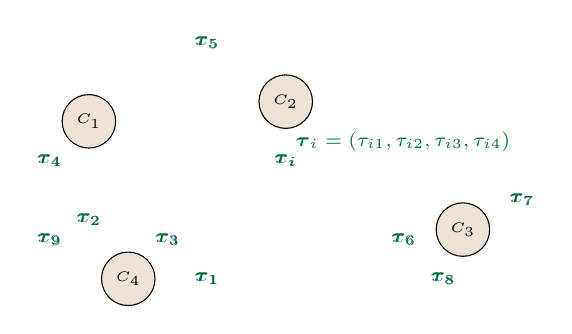
\begin{tikzpicture}[scale=0.5]
  
  %\tikzstyle{obs}   = [minimum size=1.1em]
  \tikzstyle{class} = [circle, draw, fill=class!20, minimum size=1em]
  %\tikzstyle{post}  = [ minimum size=1.8em]
  \tikzstyle{line}  = [draw, thick, -latex']

   \newcommand*{\horiz}{20}
   \newcommand*{\verti}{8}
   
   \newcommand*{\lobs}{7}
   \newcommand*{\lpost}{-1}
   \newcommand*{\osep}{14.5}
   \newcommand*{\psep}{4}

  %\draw[help lines] (0,0) grid (\horiz,\verti);
  \node<2-> (C1) [class] at(2, 5) {\tiny $C_1$};
  \node<2-> (C2) [class] at(7, 5.5) {\tiny $C_2$};
  \node<2-> (C3) [class] at(11.5, 2.25) {\tiny $C_3$};
  \node<2-> (C4) [class] at(3, 1) {\tiny $C_4$};
  
  \node<1-3> (Xi) [obs] at (7,4) {\scriptsize $x_i$};
  \node<1-4> (X2) [obs] at (2,2.5) {\scriptsize $x_2$};
  \node<1-4> (X3) [obs] at (4,2) {\scriptsize $x_3$};
  \node<1-4> (X4) [obs] at (1,4) {\scriptsize $x_4$};
  \node<1-4> (X5) [obs] at (5,7) {\scriptsize $x_5$};
  \node<1-4> (X6) [obs] at (10,2) {\scriptsize $x_6$};
  \node<1-4> (X7) [obs] at (13,3) {\scriptsize $x_7$};
  \node<1-4> (X8) [obs] at (11,1) {\scriptsize $x_8$};
  \node<1-4> (X9) [obs] at (1,2) {\scriptsize $x_9$};
  \node<1-4> (X1) [obs] at (5,1) {\scriptsize $x_{1}$};
  
  \node<3> (Ti) [post, above right] at (Xi) {\scriptsize $\boldsymbol\tau_{i} = (\tau_{i1}, \tau_{i2}, \tau_{i3}, \tau_{i4}$)};
  
  \node<4-> (Ti) [post] at (7,4) {\scriptsize $\boldsymbol\tau_i$};
  \node<5-> (T2) [post] at (2,2.5) {\scriptsize $\boldsymbol\tau_2$};
  \node<5-> (T3) [post] at (4,2) {\scriptsize $\boldsymbol\tau_3$};
  \node<5-> (T4) [post] at (1,4) {\scriptsize $\boldsymbol\tau_4$};
  \node<5-> (T5) [post] at (5,7) {\scriptsize $\boldsymbol\tau_5$};
  \node<5-> (T6) [post] at (10,2) {\scriptsize $\boldsymbol\tau_6$};
  \node<5-> (T7) [post] at (13,3) {\scriptsize $\boldsymbol\tau_7$};
  \node<5-> (T8) [post] at (11,1) {\scriptsize $\boldsymbol\tau_8$};
  \node<5-> (T9) [post] at (1,2) {\scriptsize $\boldsymbol\tau_9$};
  \node<5-> (T1) [post] at (5,1) {\scriptsize $\boldsymbol\tau_{1}$};
  
%   \node (T2) [post, above right=3] at (X2) {\scriptsize $\boldsymbol\tau_{2}$};
%   \node (T3) [post, above right=3] at (X3) {\scriptsize $\boldsymbol\tau_{3}$};
%   \node (T4) [post, above left=3] at (X4) {\scriptsize $\boldsymbol\tau_{4}$};
%   \node (T5) [post, above right=3] at (X5) {\scriptsize $\boldsymbol\tau_{5}$};
%   \node (T6) [post, above left=3] at (X6) {\scriptsize $\boldsymbol\tau_{6}$};
%   \node (T7) [post, above right=3] at (X7) {\scriptsize $\boldsymbol\tau_{7}$};
%   \node (T8) [post, below right=3] at (X8) {\scriptsize $\boldsymbol\tau_{8}$};
%   \node (T9) [post, above left=3] at (X9) {\scriptsize $\boldsymbol\tau_{9}$};
%   \node (T10) [post, below right=3] at (X10) {\scriptsize $\boldsymbol\tau_{10}$};
  %\node (C2) [class] at(\origin-\osep, \lobs) {$C_1$};
  %\node (C3) [class] at(\origin-\osep, \lobs) {$C_1$};
%     \draw (0,0) [draw=none] grid (2*\origin,8);
%     
%     \node (X1) [obs] at (\origin-\osep,\lobs) {$x_1$};
%     \node (C1) [class] at(\origin-\osep, \lobs) {$C_1$};
%     \node (Xi) [obs] at (\origin,\lobs) {$x_i$};
%     \node (Xn) [obs] at (\origin+\osep,\lobs) {$x_n$};
% 
%     \node (T11) [post] at (\origin-\psep-\osep, \lpost) {$\tau_{11}$};
%     \node (T1j)  [post] at (\origin - \osep,  \lpost) {$\tau_{1 j}$};
%     \node (T1k) [post] at (\origin+\psep-\osep, \lpost) {$\tau_{1k}$};
% 
%     \node  (Ti1) [post] at (\origin-\psep,   \lpost) {$\tau_{i1}$};
%     \node  (Tij)  [post] at (\origin, \lpost) {$\tau_{i j}$};
%     \node  (Tik) [post] at (\origin+\psep, \lpost) {$\tau_{ik}$};
% 
%     \node (Tn1) [post] at (\origin-\psep+\osep,\lpost) {$\tau_{n1}$};
%     \node (Tnj)  [post] at (\origin + \osep, \lpost) {$\tau_{n j}$};
%     \node (Tnk) [post] at (\origin+\psep+\osep, \lpost) {$\tau_{nk}$};
% 
%     \path (X1) -- (Xi) node [font=\Huge, midway, sloped] {$\dots$};
%     \path (Xi) -- (Xn) node [font=\Huge, midway, sloped] {$\dots$};
% 
%     \path[dotted] (X1) edge (T11);
%     \path[dotted] (X1) edge (T1j);
%     \path[dotted] (X1) edge (T1k);
% 
%     \path[dotted] (Xi) edge (Ti1);
%     \path[dotted] (Xi) edge (Tij);
%     \path[dotted] (Xi) edge (Tik);
% 
%     \path[dotted] (Xn) edge (Tn1);
%     \path[dotted] (Xn) edge (Tnj);
%     \path[dotted] (Xn) edge (Tnk);
\end{tikzpicture}
\end{center}
\end{frame}


\begin{frame}[t]
\frametitle{Partitioning a finite set}
\begin{block}{Partition of a finite set}
Let $I^k = \{1, \dots, k \}$ be a finite set. A \emph{partition of $I^k$}  is a set $\mathcal{I}$ of subsets of $I^k$, each subset  called part, such that 
\begin{itemize}
\item $\bigcup_{I \in \mathcal{I}} = I^k$ and 
\item $I \cap J = \emptyset$  for every $I, J \in \mathcal{I}$ different.
\end{itemize}
\end{block}

\medskip
\pause

\begin{columns}
\column{0.5\textwidth}%
For example if $I^4$
\begin{itemize}
\item $\mathcal{I} = \{ \{1, 2, 3, 4\} \}$
\item $\mathcal{I} = \{ \{1 \}, \{2, 4\}, 3 \}$
\item $\mathcal{I} = \{ \{1\}, \{2\}, \{3\}, \{4\} \}$
\end{itemize}
\column{0.5\textwidth}
\only<4>{%
For example if $F = \{H, O, L, A\}$
\begin{itemize}
\item $\mathcal{I} = \{ \{H, O, L, A \} \}$
\item $\mathcal{I} = \{ \{H \}, \{O, A \}, L \}$
\item $\mathcal{I} = \{ \{H\}, \{O \}, \{L \}, \{A \} \}$
\end{itemize}
}%
\end{columns}

\medskip
\pause
\begin{itemize}
\item[] For any finite set $F$, the partition can be defined naturally indexing its elements.
\end{itemize}
\end{frame}

\begin{frame}[t]
\frametitle{Hierarchical combination of a finite set}
\begin{block}{Hierarchical combination of a finite set}
A hierarchical combination of a finite set with $k$ elements is a sequence of partitions $\mathcal{I}_1, \mathcal{I}_2, \dots \mathcal{I}_k$ of $I^k$, such that for each i, $1 \leq i \leq k$,
\begin{itemize}
\item $\mathcal{I}_i$ has $i$ elements and
\item if a part $I \in \mathcal{I}_{i-1}$ then there is a part $J \in \mathcal{I}_i$ with $J = I$ or there are two parts $J_1, J_2 \in \mathcal{I}_i$ with $I = J_1 \cup J_2$.
\end{itemize}
\end{block}

For example,
\begin{itemize}
\item A hierarchical combination of a finite set defines a binary partition of the finite set.
\end{itemize}

\end{frame}

% Especificació del problema a resoldre.
\begin{frame}[t]
\frametitle{Our input, our goal: What do we want to do?}

\begin{block}{Input}
A sample of probabilities to belong to some classe $C_i$, 
\begin{columns}
\column{0.4\textwidth}
\[ T = \left[ \begin{array}{ccccc}
\idea{(}\tau_{11}\idea{,} & \dots & \tau_{1j}\idea{,} & \dots & \tau_{1k}\idea{),} \\
\vdots      & &    \vdots                     & &    \vdots                     \\
\idea{(}\tau_{11}\idea{,} & \dots & \tau_{1j}\idea{,} & \dots & \tau_{1k}\idea{),} \\
\vdots      & &      \vdots                   & &       \vdots                  \\
\idea{(}\tau_{11}\idea{,} & \dots & \tau_{1j}\idea{,} & \dots & \tau_{1k}\idea{)}
\end{array} \right] 
\idea{ \in \mathcal{S}_{[C_1,\dots,C_k]}^k } \]
\column{0.3\textwidth}
\end{columns}
\end{block}

\pause
\begin{alertblock}{Goal}
\alert{Merge} classes (sequentially) to obtain a hierarchy over the set of classes % $\{C_1, \dots, C_k\}$. %In other words, obtain a binary tree with a set of leafs $\{C_1, \dots, C_k\}$
\end{alertblock}
\end{frame}




\begin{frame}[t]
\frametitle{Where do $\boldsymbol\tau_i$'s come from?}

\begin{description}
\item[Expert decision] An expert set the weights according to its expertise
\item[Mixture models]  The a posteriori probabilities
\begin{eqnarray*} \tau_{ij} &=& \frac{f(x_i; \theta_j)}{\sum_{\ell = 1}^k f(x_i; \theta_\ell) } \end{eqnarray*}
\item[Fuzzy clustering] The membership weight \uncover<2->{ (if $f'(x; C) := \frac{1}{d(x, C)}^{2/(m-1)}$)  }
\begin{eqnarray*}
\tau_{ij} &=& \frac{1}{\sum_{\ell = 1}^k \left( \frac{d(x_i; C_j)}{d(x_i; C_\ell) } \right)^{2/(m-1)}}  \\
\uncover<3>{ &=& \frac{f'(x_i; C_j)}{\sum_{\ell = 1}^k f'(x_i; C_\ell)} }
\end{eqnarray*}
\end{description}
\end{frame}




%%% Mixture models
\section{Merging classes: mixture models}

\begin{frame}
\frametitle{Mixture models: obtaining the a posteriori probabilities}
\begin{itemize}
\item A sample $X= \{\textbf{x}_1, \dots, \textbf{x}_i, \dots, \textbf{x}_n\}$.
\item<2-> A fitted mixture model with $k$ components $C_j$, $1 \leq j \leq k$.
\item<3-> $\tau_{ij} = P( \left\{ \textbf{x}_i \in C_j \right\})$, $1 \leq i \leq n$ and $1 \leq j \leq k$.
\end{itemize}
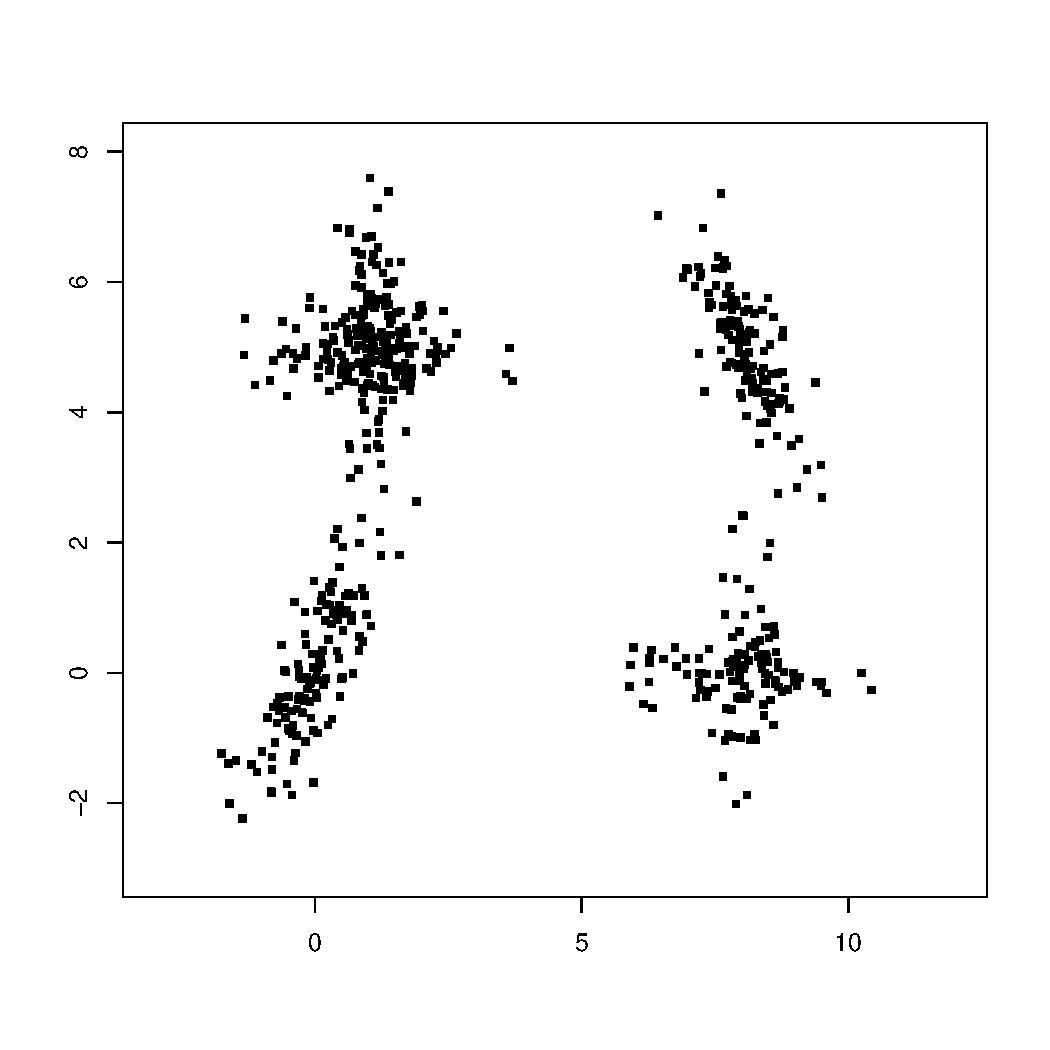
\includegraphics[width=0.33\textwidth]{data41.pdf}
\visible<2->{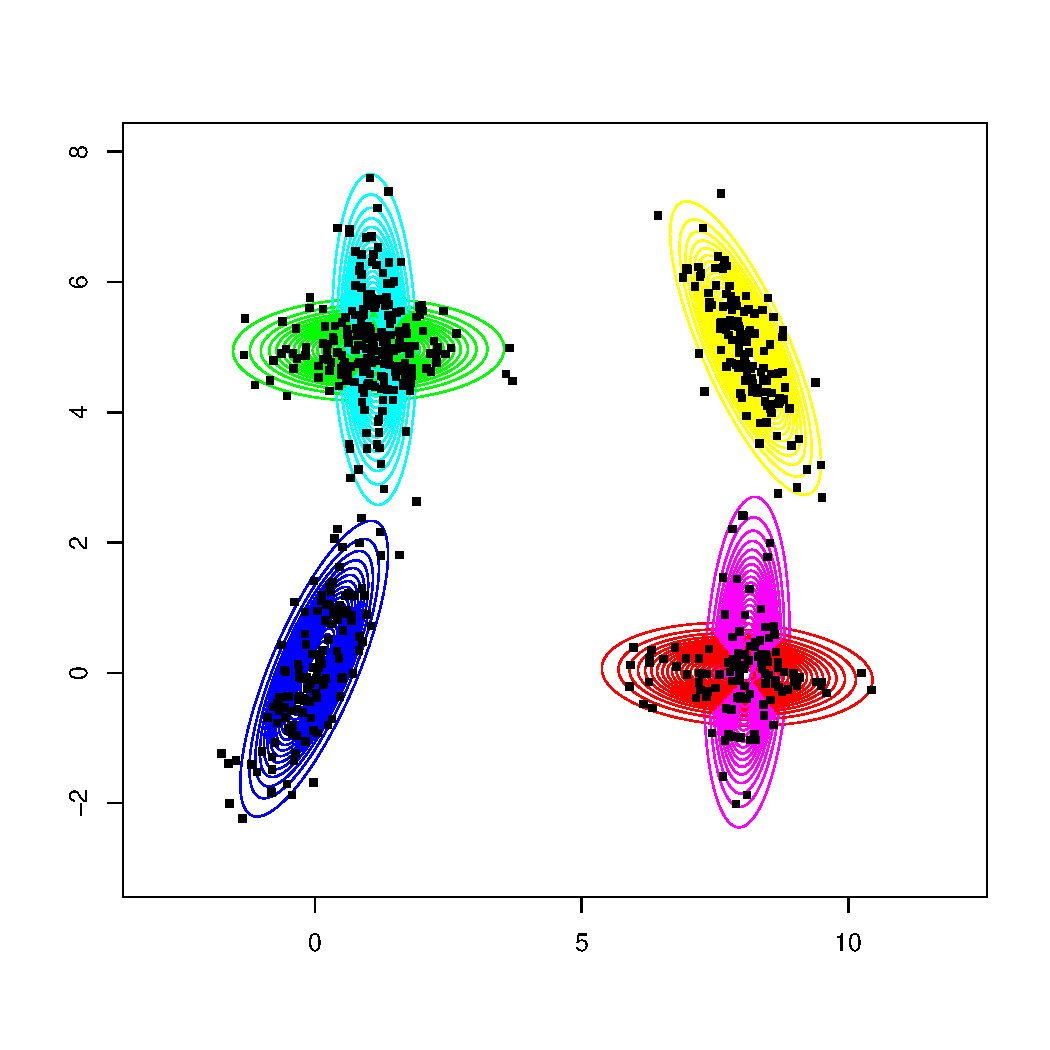
\includegraphics[width=0.33\textwidth]{data41dist.pdf}}
\visible<3->{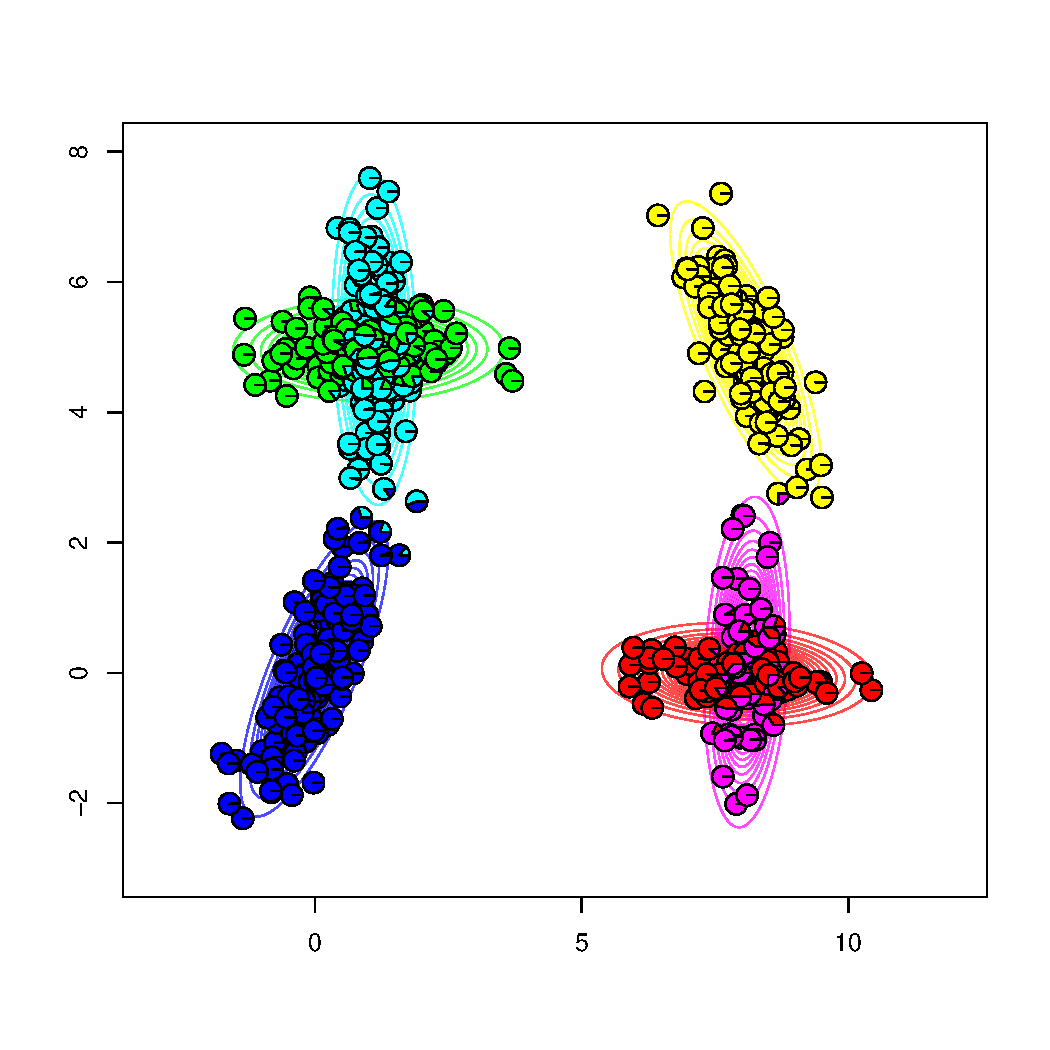
\includegraphics[width=0.33\textwidth]{data41posteriori.pdf}}
\end{frame}

\begin{frame}[t]
\frametitle{Whats does "merge" usually mean  in mixture modeling?}
\begin{itemize}
\item Merging class $C_a$ with class $C_b$ to a new class $C_c$ means that observation related to class $C_{ab}$ either is related to class $C_a$ or to class $C_b$.
\item Mixture models assume that an observation comes from a unique component (belongs to a unique class).
\item For an observation $\textbf{x}_i$ 
\begin{eqnarray*} 
\uncover<2>{ \tau_{i c}  \;=\;} P( \{ \textbf{x}_i \in C_{c} \})  &=& P( \{ \textbf{x}_i \in C_{a} \} \cup \{ \textbf{x}_i \in C_{b} \} ) \\
&=& P( \{ \textbf{x}_i \in C_{a} \}) + P( \{ \textbf{x}_i \in C_{b} \} )  \uncover<2>{ \;=\; \tau_{i a} + \tau_{i b} }
\end{eqnarray*} 
\end{itemize}
\end{frame}

\begin{frame}[t]
\frametitle{Entropy approach}
\begin{block}{Entropy approach (Baudry et~al., 2010)}
The classes to be merged are those that maximize the entropy of a posteriori probabilities
\end{block}
\small
\only<1-2>{
\uncover<2>{Maximize}
\[
\overbrace{ 
\uncover<2>{-\left(} \sum_{i=1}^n \left\{ \tau_{iI_a} \log(\tau_{iI_a}) + \tau_{iI_b} \log(\tau_{iI_b})\right\} + \sum_{i=1}^n \sum_{\substack{\ell = 1\\\ell \neq a,b}}^k  \tau_{iI_\ell} \log(\tau_{iI_\ell}) \uncover<2>{\right)+}
}^{
\substack{\text{entropy }\\\text{before merging}}  
} 
\]
\[
\underbrace{ 
\uncover<2>{+\left( } \sum_{i=1}^n  (\tau_{iI_a}+\tau_{iI_b}) \log(\tau_{iI_a} + \tau_{iI_b}) + \sum_{i=1}^n  \sum_{\substack{\ell = 1\\\ell \neq a,b}}^k  \tau_{iI_\ell} \log(\tau_{iI_\ell}) \uncover<2>{\right)}
}_{
\substack{\text{entropy }\\\text{after merging}}   
} 
\]
}
\only<3>{
Maximize
\[
- \sum_{i=1}^n \left\{ \tau_{iI_a} \log(\tau_{iI_a}) + \tau_{iI_b} \log(\tau_{iI_b})\right\} + \sum_{i=1}^n  (\tau_{iI_a}+\tau_{iI_b}) \log(\tau_{iI_a} + \tau_{iI_b})
\]
}
%\only<4>{
%Minimize
%\[
% \sum_{i=1}^n \left\{ \tau_{iI_a} \log(\tau_{iI_a}) + \tau_{iI_b} \log(\tau_{iI_b})\right\} - \sum_{i=1}^n  (\tau_{iI_a}+\tau_{iI_b}) \log(\tau_{iI_a} + \tau_{iI_b})
%\]
%}
\end{frame}

\begin{frame}
\frametitle{Summarizing}

\begin{itemize}
\item How to combine?
\begin{itemize}
\item Amalgamation:
\item Geometric mean: ${\boldsymbol\tau}^{\mathcal{I}}_i$
\end{itemize}
\item How to evaluate the combination of $a$and $b$?
\[ \frac{  
  \mathlarger\sum_{i=1}^n
		\omega ({\boldsymbol\tau}^{\mathcal{I}}_i, a) \cdot
		\theta ({\boldsymbol\tau}^{\mathcal{I}}_i, a, b)
}{  
	\mathlarger\sum_{i=1}^n  
		\omega ({\boldsymbol\tau}^{\mathcal{I}}_i, a) 
}, \]
\end{itemize}
\end{frame}

\begin{frame}
\frametitle{Methods}
\begin{itemize}
\item Methods based on modality
\begin{itemize}
\item The ridgeline unimodal method
\end{itemize}
\item Methods based on misclafication probabilities
\begin{itemize}
\item Bhattacharyya distance method
\item Entropy approach
\item Directly estimated misclassification probabilities
\end{itemize}
\end{itemize}
\end{frame}


\begin{frame}
\frametitle{Entropy approach}
\end{frame}

\begin{frame}
\frametitle{Directly estimated misclassification \\probabilities (DEMP)}
\end{frame}


%%% Further work
\section{Merging classes: going further}

\begin{frame}
\frametitle{Whats does "merge" usually mean  in general?}
%\frametitle{Merging operation}


\begin{itemize}
\item What if we apply geometric mean instead of amalgamation
\end{itemize}
\end{frame}

\begin{frame}
\frametitle{Ideas}
\begin{itemize}
\item Usually, we assume our sample $X$ to be near to the center of a class. Is this assumption really important to merge clusters?
\end{itemize}
\end{frame}

\begin{frame}[t]
\frametitle{Fuzzy clustering VS Mixture modeling}

% \begin{columns}
% \column{0.5\textwidth}
% \begin{itemize}
% \item 
% \end{itemize}
% \column{0.5\textwidth}
% \begin{itemize}
% \item 
% \end{itemize}
% \end{columns}

\begin{columns}
\column{0.5\textwidth}
Fuzzy-clustering\medskip
\begin{itemize}
\item Initialize $(\omega_{i1}^0, \dots, \omega_{ik}^0)$.
\end{itemize}
\column{0.5\textwidth}

Gaussian mixture modeling\medskip
\begin{itemize}
\item Initialize $(\tau_{i1}^0, \dots, \tau_{ik}^0)$.
\end{itemize}
\end{columns}

\begin{columns}
\column{0.5\textwidth}
\begin{itemize}
\item $c^{\ell+1}_j = \frac{\sum_{i=1}^n \omega_{i j}^{\red{m}} \obs{x_i}}{\sum_{i=1}^n \omega_{i j}^{\red{m}}}$
\end{itemize}
\column{0.5\textwidth}
\begin{itemize}
\item $\mu^{\ell+1}_j = \frac{\sum_{i=1}^n \tau_{i j} \obs{x_i}}{\sum_{i=1}^n \tau_{i j}}$
\end{itemize}
\end{columns}

\begin{columns}
\column{0.5\textwidth}
\begin{itemize}
\item $\omega^{\ell+1}_{ij} = \frac{1}{\sum_{\ell = 1}^k \left( \frac{d(x_i; C_j)}{d(x_i; C_\ell) } \right)^{2/({\red{m}}-1)}}$
\end{itemize}
\column{0.5\textwidth}
\begin{itemize}
\item $\tau^{\ell+1}_{ij} = \frac{f(x_i; \mu_j, \Sigma_\ell)}{\sum_{\ell = 1}^k f(x_i; \mu_\ell, \Sigma_\ell) }$
\end{itemize}
\end{columns}


\end{frame}
\end{document}